% Section of thesis on DUNE 35ton prototype
% Target: 30 pages

\graphicspath{{35ton/Figs/}}

\chapter{The DUNE 35~ton Prototype}\label{chap:35ton}

The 35~ton is the first experimental prototype of the DUNE far detector design and was briefly introduced in Section~\ref{sec:RoadToDUNE}.  It was originally constructed to demonstrate the unique design features of the LBNE far detector and was the only planned prototype for this experiment.  Following the dissolution of LBNE and the subsequent formation of the DUNE collaboration, the 35~ton has become an integral part of the design and execution of the DUNE far detector design.

As discussed in Section~\ref{sec:LArTPC}, the use of LArTPCs in future long-baseline experiments shows great promise.  To facilitate development of the detector technology, Fermilab has an extensive program of LArTPC experiments culminating in the flagship DUNE project.  Prototying is essential to the success of DUNE as understanding of how to operate progressively larger detectors evolves.  The stategy is staged, with each subsequent phase building on previous success.

The most pertinent issues facing large-scale LArTPCs concern:
\begin{itemize}
  \item the ability to achieve and maintain the necessary LAr purity for successful data taking;
  \item the design and construction of huge underground cryostats.
\end{itemize}
The research and development performed thus far have demonstrated viable solutions to these obstacles and has resulted in the situation where ProtoDUNE can be attempted with confidence.

The outcomes of each of these projects at Fermilab are the subject of this present chapter.  The first of the above issues, regarding LAr purity, is discussed in Section~\ref{sec:MTSLAPD} with reference to the Materials Test Stand and the Liquid Argon Purity Demonstrator.  The second complication, concerning the construction of large underground cryostats, was the main motivation for the 35~ton Phase~I experiment and is the subject of Section~\ref{sec:35tonPhaseI}.  The culmination of all these developments involved operating a small scale LArTPC alongside these improvements and was achieved in the 35~ton Phase~II run, discussed in Section~\ref{sec:35tonPhaseII}.  Since this experiment forms the basis for later chapters, it will be reviewed in much greater detail.  A summary of all this R\&D is presented in Section~\ref{sec:35tonSummary}.

\section[The Materials Test Stand and Liquid Argon Purity Demonstrator]{The Materials Test Stand and\\Liquid Argon Purity Demonstrator}\label{sec:MTSLAPD}

The work on developing LArTPCs for future neutrino experiments began at FNAL in 2007 with a view to eventually facilitating a multi-kton LAr experiment.  Even utilising a modular design, as with the DUNE far detector (Section~\ref{sec:FarDetector}), drift distances on the order of a few metres are realistically required, necessitating a low concentration of electronegative impurities.  Attaining and holding the requisite LAr purity in a huge underground cryostat over many years of running is a considerable challenge addressed by the test stands reviewed in this section.

\subsection{The Materials Test Stand}\label{sec:MTS}

The Materials Test Stand (MTS) \cite{MTS2006,MTS2009a,MTS2009b,MTS2011} was constructed at FNAL to develop LAr purification techniques and to characterise the effect of various materials on the electron lifetime when submerged in the liquid.  It consists of a small cryostat and two filters containing activated-copper-coated granules and an adsorbent molecular sieve respectively; a schematic of the MTS setup is shown in Figure~\ref{fig:MTS}.  The filters are designed to remove oxygen and water contaminants with functionality similar to that successfully demonstrated by the ICARUS collaboration \cite{ICARUS1993b}.  Oxygen is removed by the copper beads using the chemical reaction
\begin{equation}
  2~\textnormal{Cu} + \textnormal{O}_2 \rightarrow 2~\textnormal{CuO}
\end{equation}
and water molecules are physically trapped in the microporous structure of the sieve.  The filters additionally contain the ability to be regenerated in situ, a necessity when planning a long-running experiment, multi-kton experiment; those used previously were primarily proprietary \cite{ICARUS1993a,ICARUS2006}.

\begin{figure}
  \centering
  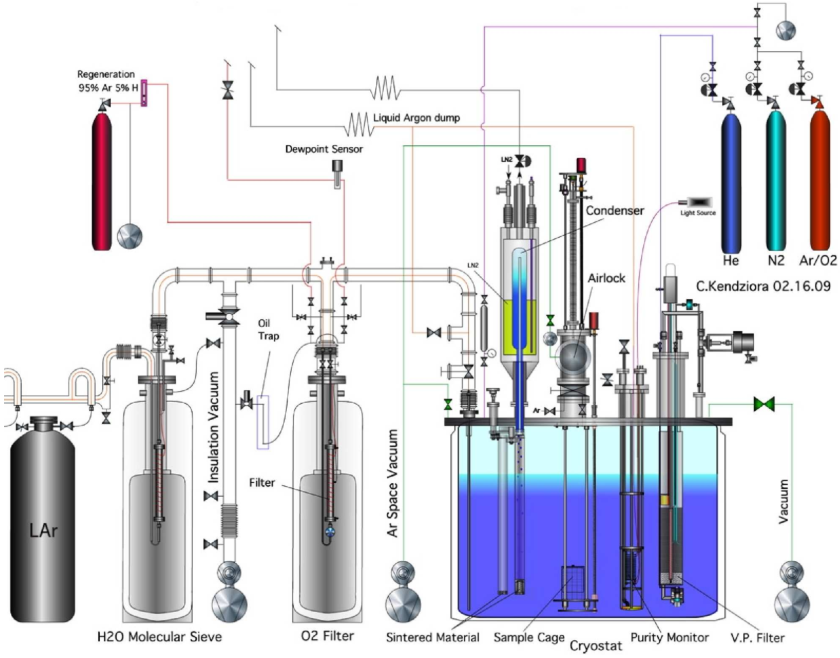
\includegraphics[width=14cm]{MTS.pdf}
  \caption[The Materials Test Stand Stand at FNAL.]{The Materials Test Stand Stand at FNAL \cite{MTS2009b}.  Liquid argon used to fill the cryostat flows from left to right in the schematic, through two filters designed to reduce the H$_2$O and O$_2$ contamination respectively.  A second filter system (the `vapour pump' (V.P.)), using the same materials, is installed within the cryostat to remove impurities introduced by the materials being examined.}
  \label{fig:MTS}
\end{figure}

The MTS successfully demonstrated good argon purity ($<3$~ppb~H$_2$O) and showed the primary opposition to electron lifetime is water contamination, demonstrated in Figure~\ref{fig:MTSResults}.  It was found that exposure to warm surfaces in the cryostat, such as above the liquid level, facilitated contamination from water impurities as they remain on surfaces even in a vacuum.  The condenser used in the MTS to recondense gaseous argon returned it directly to the liquid in the cryostat (as `raining' condensation) and was found to dramatically reduce the LAr purity when in use.  This is due to contaminants introduced into the gas by exposure to the warm croystat walls which could be negated by returning the liquid via a different path which maximised subjection to cold surfaces.  Notably, the electron lifetime was found to be unaffected on the introduction of test materials, although as suspected the temperature of the materials did have an impact.  This is a hugely promising result for the future of LArTPC design and construction.

\begin{figure}
  \centering
  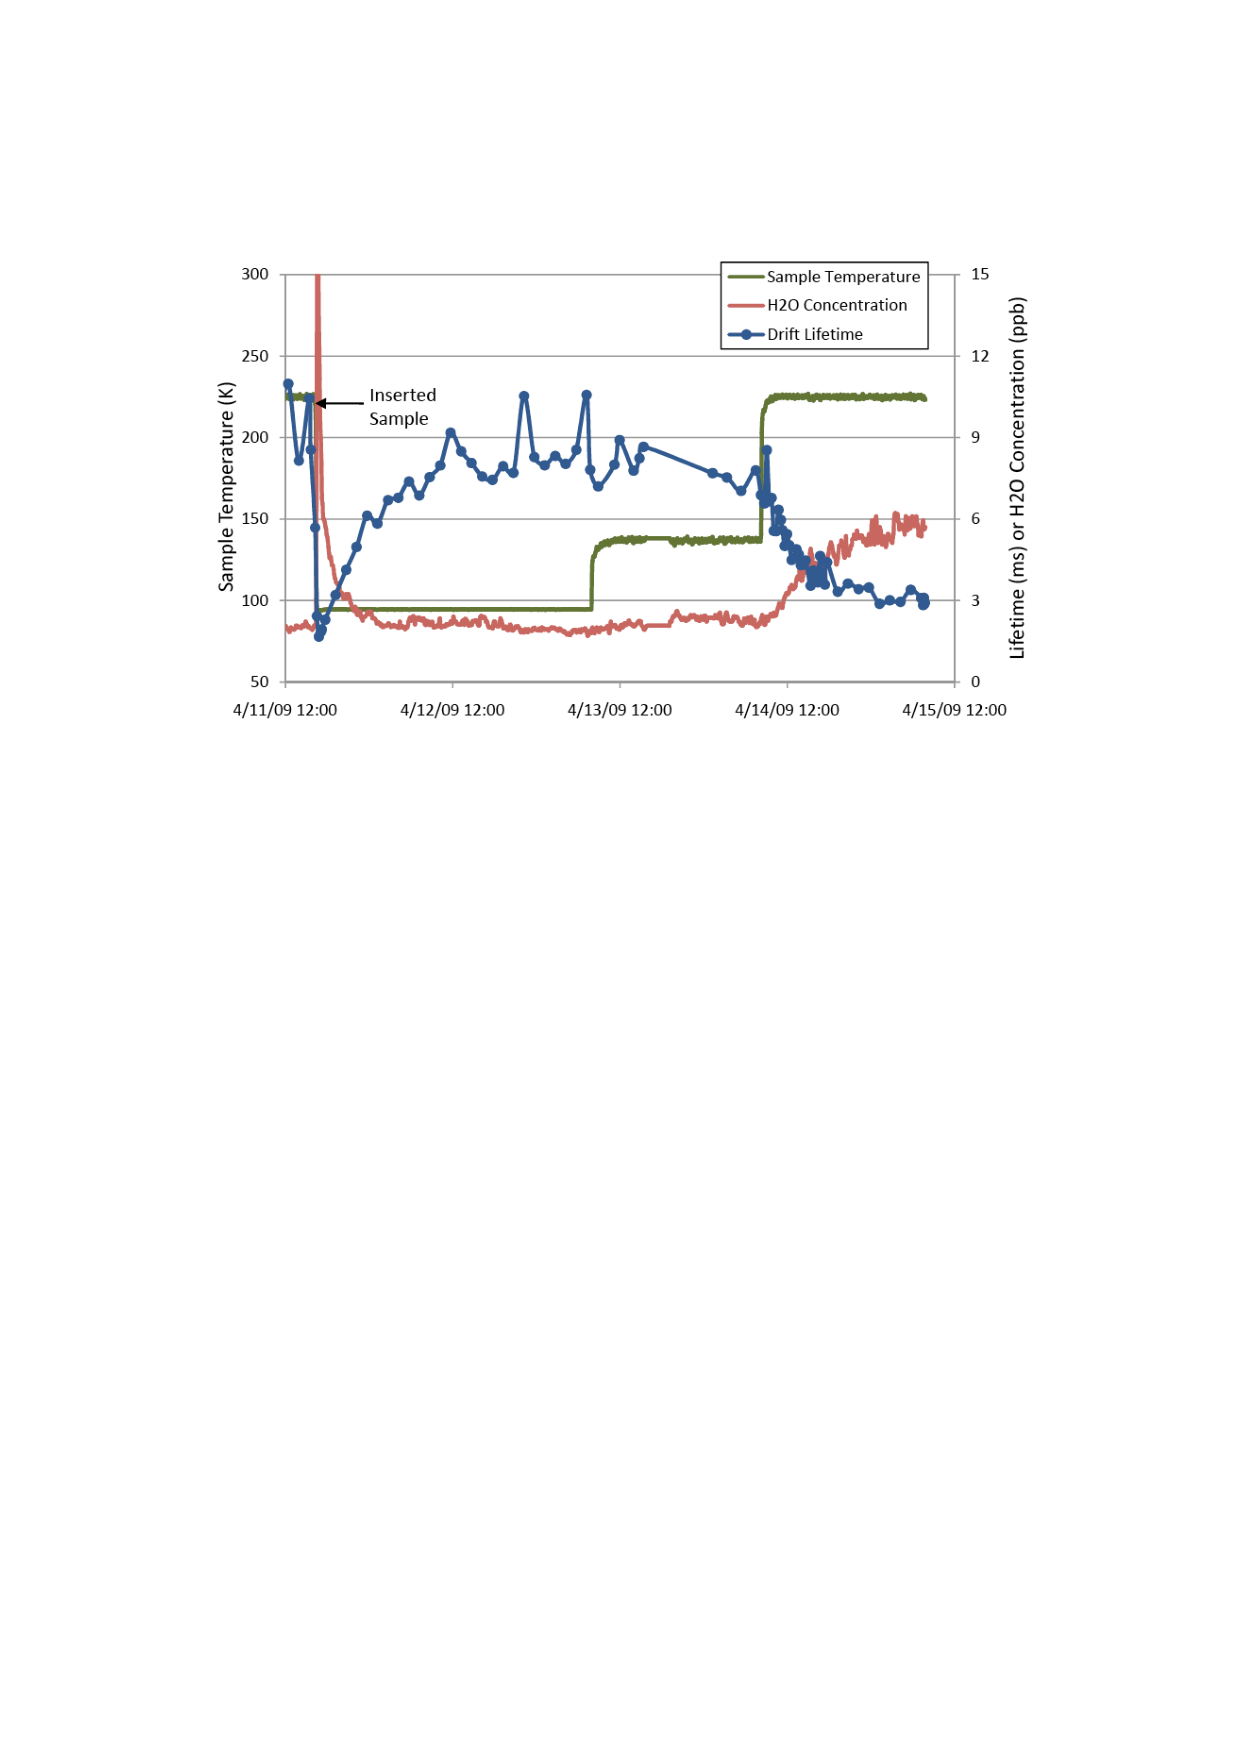
\includegraphics[width=12cm]{MTSResults.pdf}
  \caption[Results from the Materials Test Stand showing the water contamination in LAr and the corresponding electron lifetime.]{Results from the Materials Test Stand showing the water contamination in LAr and the corresponding electron lifetime \cite{MTS2009a}.  There is an obvious inverse correlation between the density of electronegative (H$_2$O) impurities and the resulting lifetime.}
  \label{fig:MTSResults}
\end{figure}

\subsubsection{Filter Regeneration}\label{sec:FilterRegeneration}

Over time, the filters become less effective as electronegative impurities accumulate.  A significant success of the MTS was demonstrating the process of regenerating the filters in situ.  This is achieved by heating the vessels to 250$^{\circ}$C and, in the case of the molecular sieve, simply using a vacuum pump to remove the water vapour or, in the case of the activated copper, by pumping through a 95:5 mixture of Ar:H$_2$ gas to capture the oxygen through the reduction reaction
\begin{equation}
  \textnormal{CuO} + \textnormal{H}_2 \rightarrow \textnormal{Cu} + \textnormal{H}_2\textnormal{O}.
\end{equation}
During the running of the test stand, the filters were regenerated after the passage of around 1000~litres of liquid argon.

\subsubsection{Purity Monitoring}\label{sec:PurityMonitoring}

The ability to constantly evaluate the LAr purity during an experimental run is hugely important to ensure high quality data.  The impurity concentrations are typically beyond the capabilities of many conventional gas analysers and so a custom device, known as a `purity monitor' (PrM), is utilised.  The design is based on the purity monitors developed by ICARUS \cite{ICARUSPurityMonitor} and is shown in Figure~\ref{fig:PurityMonitor}.

\begin{figure}
  \centering
  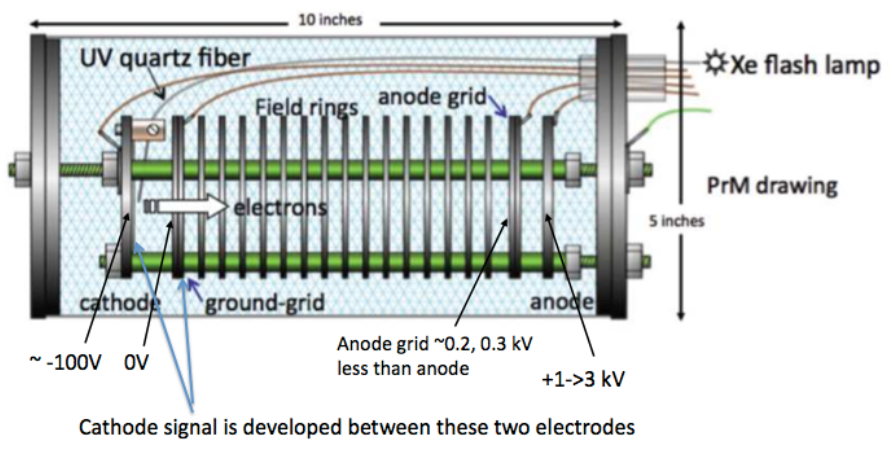
\includegraphics[width=10cm]{PurityMonitor.png}
  \caption[Schematic design of the purity monitors utilised at the FNAL LAr test stands.]{Schematic design of the purity monitors utilised at the FNAL LAr test stands \cite{}.  Purity monitors using this design were pioneered by ICARUS \cite{ICARUSPurityMonitor} and used in the MTS along with the subsequent Liquid Argon Purity Demonstrator (Section~\ref{sec:LAPD}) and 35~ton Runs I (Section~\ref{sec:35tonPhaseI}) and II (Section~\ref{sec:35tonPhaseII}).}
  \label{fig:PurityMonitor}
\end{figure}

The PrM consists of a cylindrical volume containing LAr from its surrounding environment and an anode and photocathode separated by a short drift region.  When taking purity measurments, light from a Xenon flash lamp is incident on the cathode, liberating photoelectrons which traverse towards the anode.  Electronegative impurities in the LAr will decrease the electron lifetime and therefore the number of electrons reaching a certain point along the drift volume.  A measurement of the ratio of the charge arriving at the anode to that at the cathode is hence a measurement of the inherit purity of the liquid.

The MTS cryostat contains a purity monitor and they were subsequently used in the Liquid Argon Purity Demonstrator and the 35~ton.  When developed for the Liquid Argon Purity Demonstrator and 35~ton cryostats, two sizes were used; long (47~cm) and short (16~cm).

\subsection{The Liquid Argon Purity Demonstrator}\label{sec:LAPD}

The Liquid Argon Purity Demonstrator (LAPD) \cite{MTS2011,LAPD2014,LAPDJINST2014} was designed to demonstrate the required purity of LArTPC experiments is possible without the use of large scale vacuum pumps.  Previous and current LArTPC experiments, such as ICARUS, Argoneut, LArIAT and MicroBooNE, have been constructed as flat plane vessels and have used an evacuation method as the first step in removing atmospheric impurities to facilitate the required LAr purity.  The necessary mechanical capability of the cryostat to withstand this process, along with the associated equipment, results in unfeasible engineering challenges and costs as detectors increase to multi-kton scales.

In order to circumvent these issues, a design utilising multiple smaller-scale cryostats was proposed.  This however leads to greater complexity relating to both the engineering requirements of the piping infrastructure and the reconstruction capabilities of interactions spanning multiple active volumes.  LAPD successfully pioneering an alternative approach, using a `piston purge' as a first purification step to remove atmospheric impurities.  This is a hugely important result and has significantly influenced the design of future LArTPC experiments, including the 35~ton.  Additionally, although designed to be evacuated with vacuum pumps, MicroBooNE was filled using the piston purge technique following the success of LAPD.

\subsubsection{LAPD Experimental Setup}\label{sec:LAPDExperimentalSetup}

The LAPD cryostat is shown in Figure~\ref{fig:LAPD}.  It consists of a cylindrical tank, diameter 10~feet and height 10~feet, with a domed head capable of holding 32.6~ton LAr.  It is physically next to the MTS and uses the purification system prototyped by this previous effort.  Insulation for the tank is provided by fibreglass sheets covering the outer volume which, along with the tank, is refrigerated by liquid nitrogen (LN$_2$) from an external supply.  As with the MTS, a condenser is utilised above the croystat to recondense argon gas using coils also cooled with LN$_2$.  This liquid is subsequently sent through the filtration system before being returned to the main volume, a consequense of the previous R\&D with the MTS.  After filling, the system is closed and a good LAr purity is maintained by constant circulation of the cryostat content through the filters.

The system is instrumented with PrMs, gas analysers and temperature sensors.  Four PrMs are contained within the cryostat to measure the purity gradient with an additional one just after the filters to sample to liquid before it is returned to the main volume.  Along with purity, the temperature gradient is measured in order to study the effect of this on electron drift velocity.  The contaminants in the LAr are quantified using nitrogen, oxygen and water analysers outside of the main volume.

\begin{figure}
  \centering
  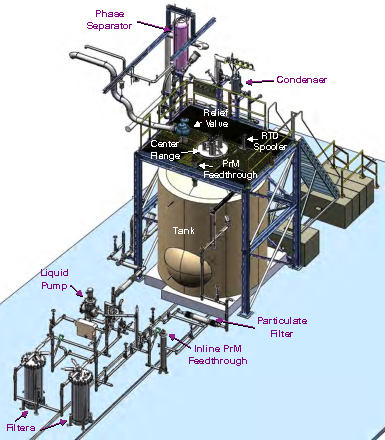
\includegraphics[width=10cm]{LAPD.pdf}
  \caption[The Liquid Argon Purity Demonstrator cryostat and purification system.]{The Liquid Argon Purity Demonstrator cryostat and purification system \cite{LAPDJINST2014}.The two cylinders at the bottom left are the filters described in Section~\ref{sec:MTS}.  The piping facilitates the transport of LAr into and out of the cryostat so continual purification within a closed system may be achieved.}
  \label{fig:LAPD}
\end{figure}

\subsubsection{Filling LAPD}\label{sec:FillingLAPD}

The piston purge technique involves injecting warm argon gas at high pressure at the bottom of the cryostat with the top open for venting, demonstrated in Figure~\ref{fig:LAPDPistonPurgeSchematic}.  The heavier than air argon gas acts as a piston, forcing the ambient air out of the top of the cryostat.  Figure~\ref{fig:LAPDPistonPurgeImpurities} demonstrates how this successfully reduces the impurity concentration in the cryostat, shown as a function of complete volume changes.  After completion of the piston purging, the O$_2$ contamination had decreased from 21\% to 6~ppm, N$_2$ from 78\% to 18~ppm and H$_2$O from 200~ppm to 1.2~ppm.

\newsavebox{\largestimage}

\begin{figure}
  \centering
  %\savebox{\largestimage}{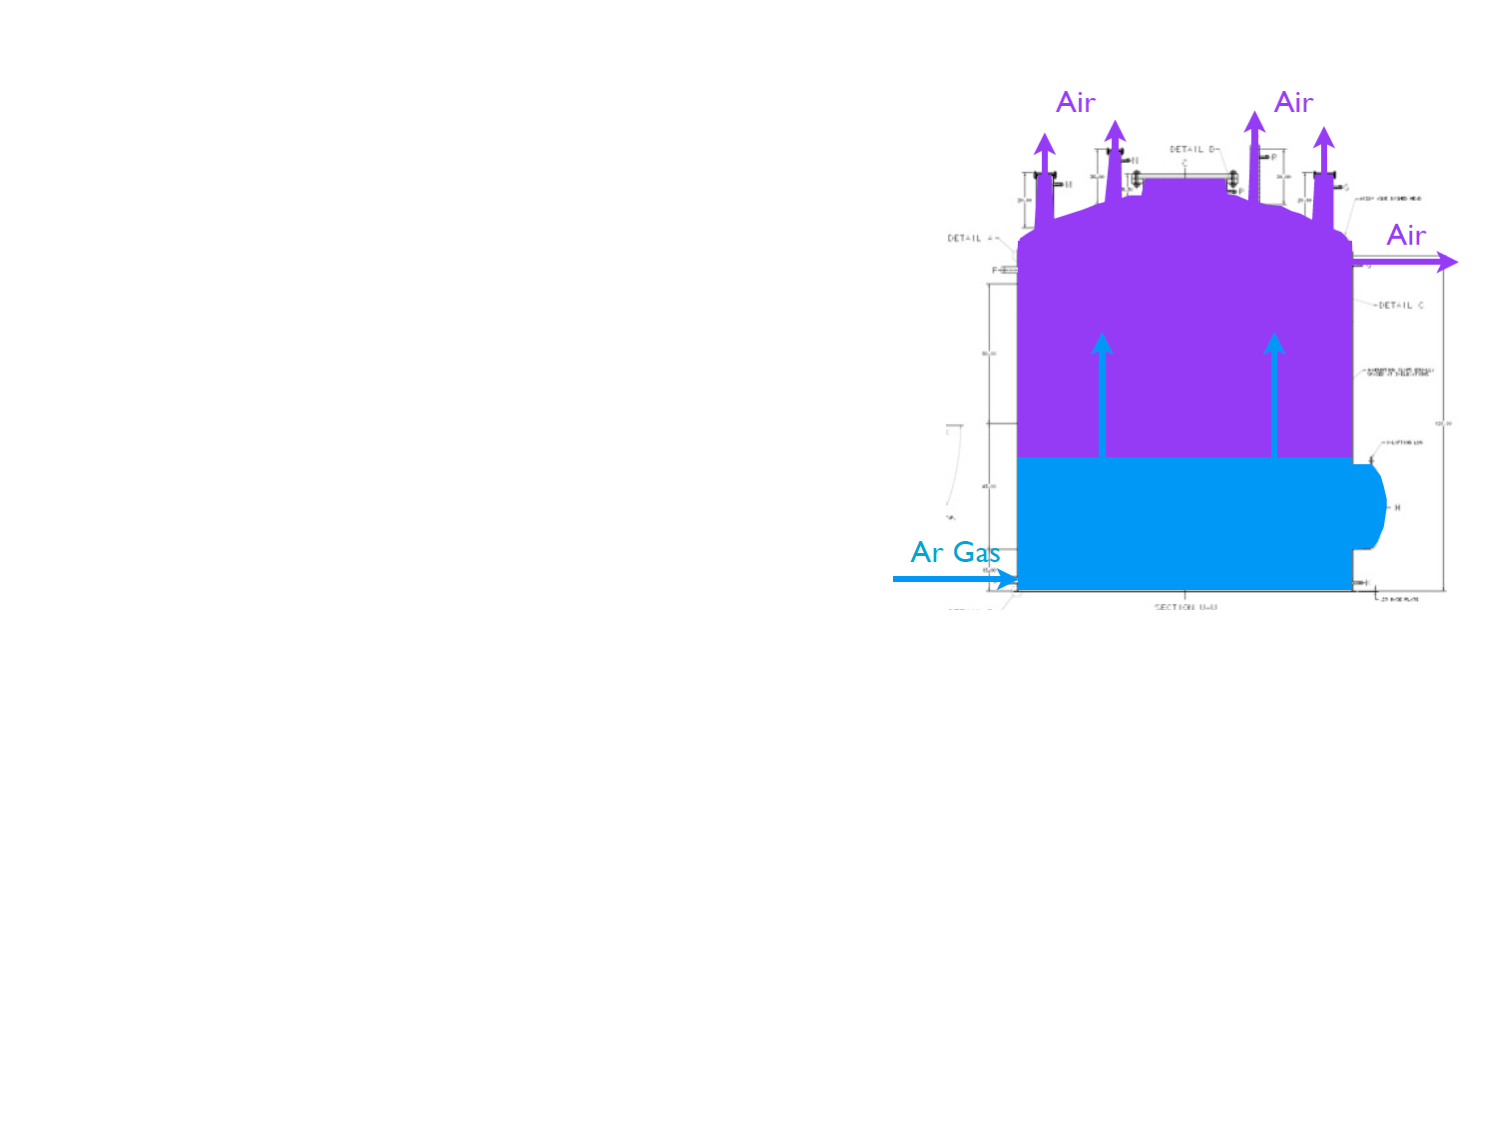
\includegraphics[width=0.49\textwidth]{LAPDPistonPurgeSchematic.pdf}}
  \begin{subfigure}[t]{0.5\linewidth}
    \centering
    %\usebox{\largestimage}
    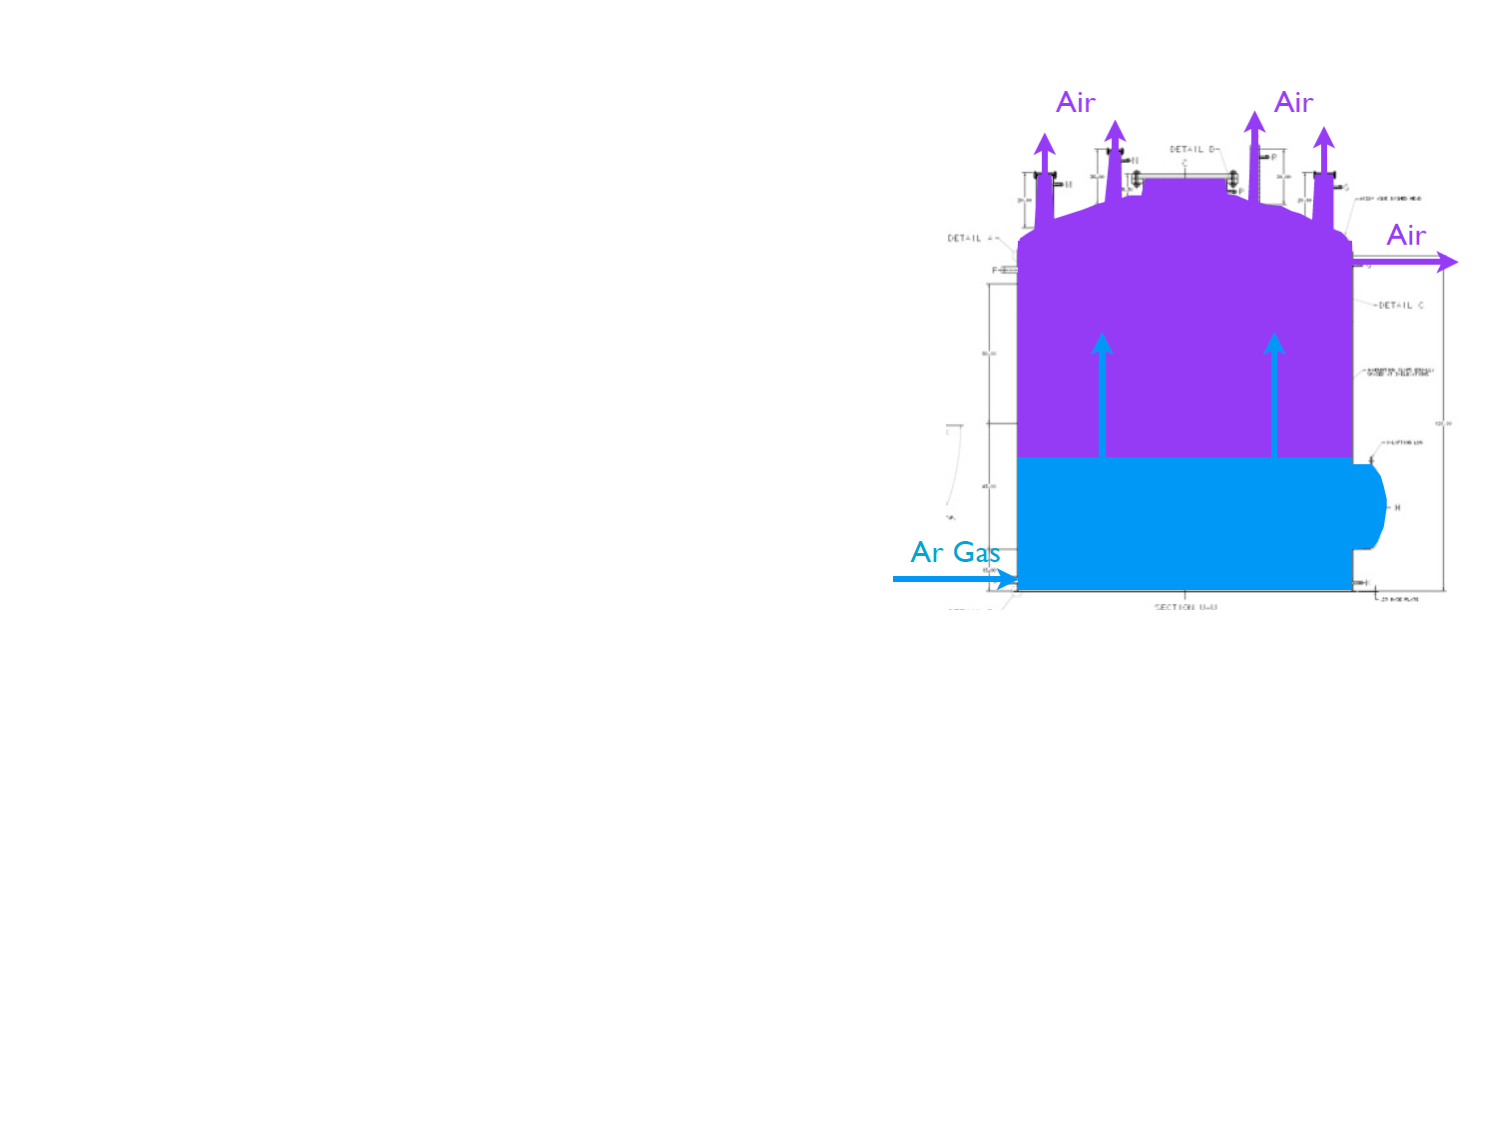
\includegraphics[width=0.98\textwidth]{LAPDPistonPurgeSchematic.pdf}
    \caption{Schematic of the LAPD piston purge.}
    \label{fig:LAPDPistonPurgeSchematic}
  \end{subfigure}\vspace{5mm}
  \begin{subfigure}[t]{0.7\linewidth}
    \centering
    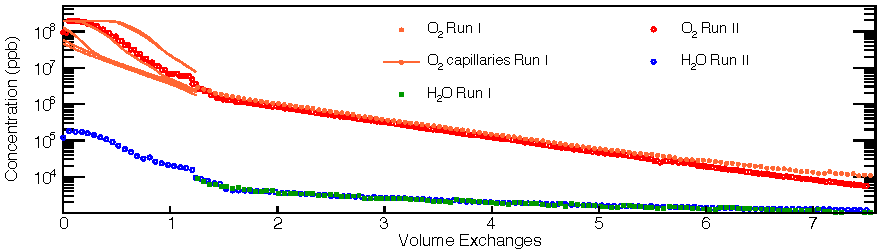
\includegraphics[width=0.98\textwidth]{LAPDPistonPurgeImpurities.pdf}
    %\raisebox{\dimexpr.5\ht\largestimage-.5\height}{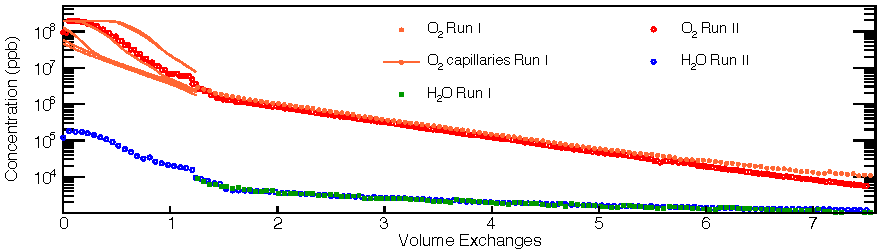
\includegraphics[width=\textwidth]{LAPDPistonPurgeImpurities.pdf}}
    \caption{LAPD impurity concentration during the piston purge.}
    \label{fig:LAPDPistonPurgeImpurities}
  \end{subfigure}
  \caption[The piston purge technique in the Liquid Argon Purity Demonstrator to remove atmopheric impurities before filling.]{The piston purge technique in the Liquid Argon Purity Demonstrator to remove atmopheric impurities before filling \cite{LAPDJINST2014}.  The results from two LAPD runs are shown, the first with the cryostat only half filled to prototype the technique.  Discontinuities between the impurity concentrations are caused by switches between gas analysers.}
  \label{fig:LAPDPistonPurge}
\end{figure}

Following the filling of the cryostat with gaseous argon, the contents are then continually circulated through the filters to further reduce the impurities present.  The improved electronegative concentrations are shown, again with reference to the number of complete volume changes, in Figure~\ref{fig:LAPDGasCirculation}.  This lasted, as can also be observed in the figure, for a number of days and resulted in a much improved O$_2$ contamination of around 20~ppb and an H$_2$O level which balanced the outgassing rate from the warm cryostat surfaces.

\begin{figure}
  \centering
  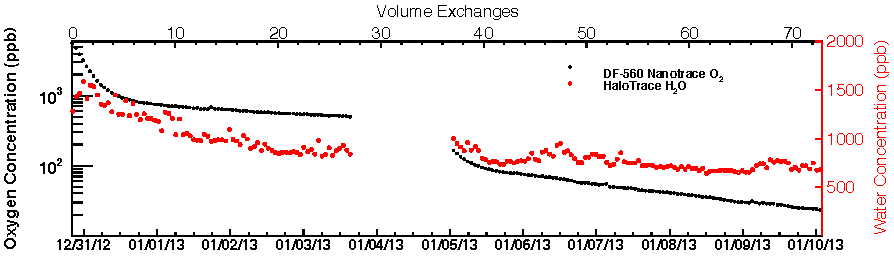
\includegraphics[width=0.7\linewidth]{LAPDGasCirculation.pdf}
  \caption[The concentration of electronegative impurities during the gas circulation stage in the Liquid Argon Purity Demonstrator following the piston purge.]{The concentration of electronegative impurities during the gas circulation stage in the Liquid Argon Purity Demonstrator following the piston purge \cite{LAPDJINST2014}.  The stabilisation of the oxygen contamination signified a leak, which was fixed during the break in readings.}
  \label{fig:LAPDGasCirculation}
\end{figure}

The filling can thus proceed by transporting LAr through the filter system into the cryostat to ensure a high purity in maintained.  The impurity concetrations were inspected before filling and after filtration and in total, a volume of 29.7~tons LAr was supplied to the LAPD cryostat.  Once filled, and during the course of operations, the liquid argon volume was constantly recirculated through the filtration system to preserve the LAr purity.  This is shown schematically in Figure~\ref{fig:LAPDLiquidCirculation}.

\begin{figure}
  \centering
  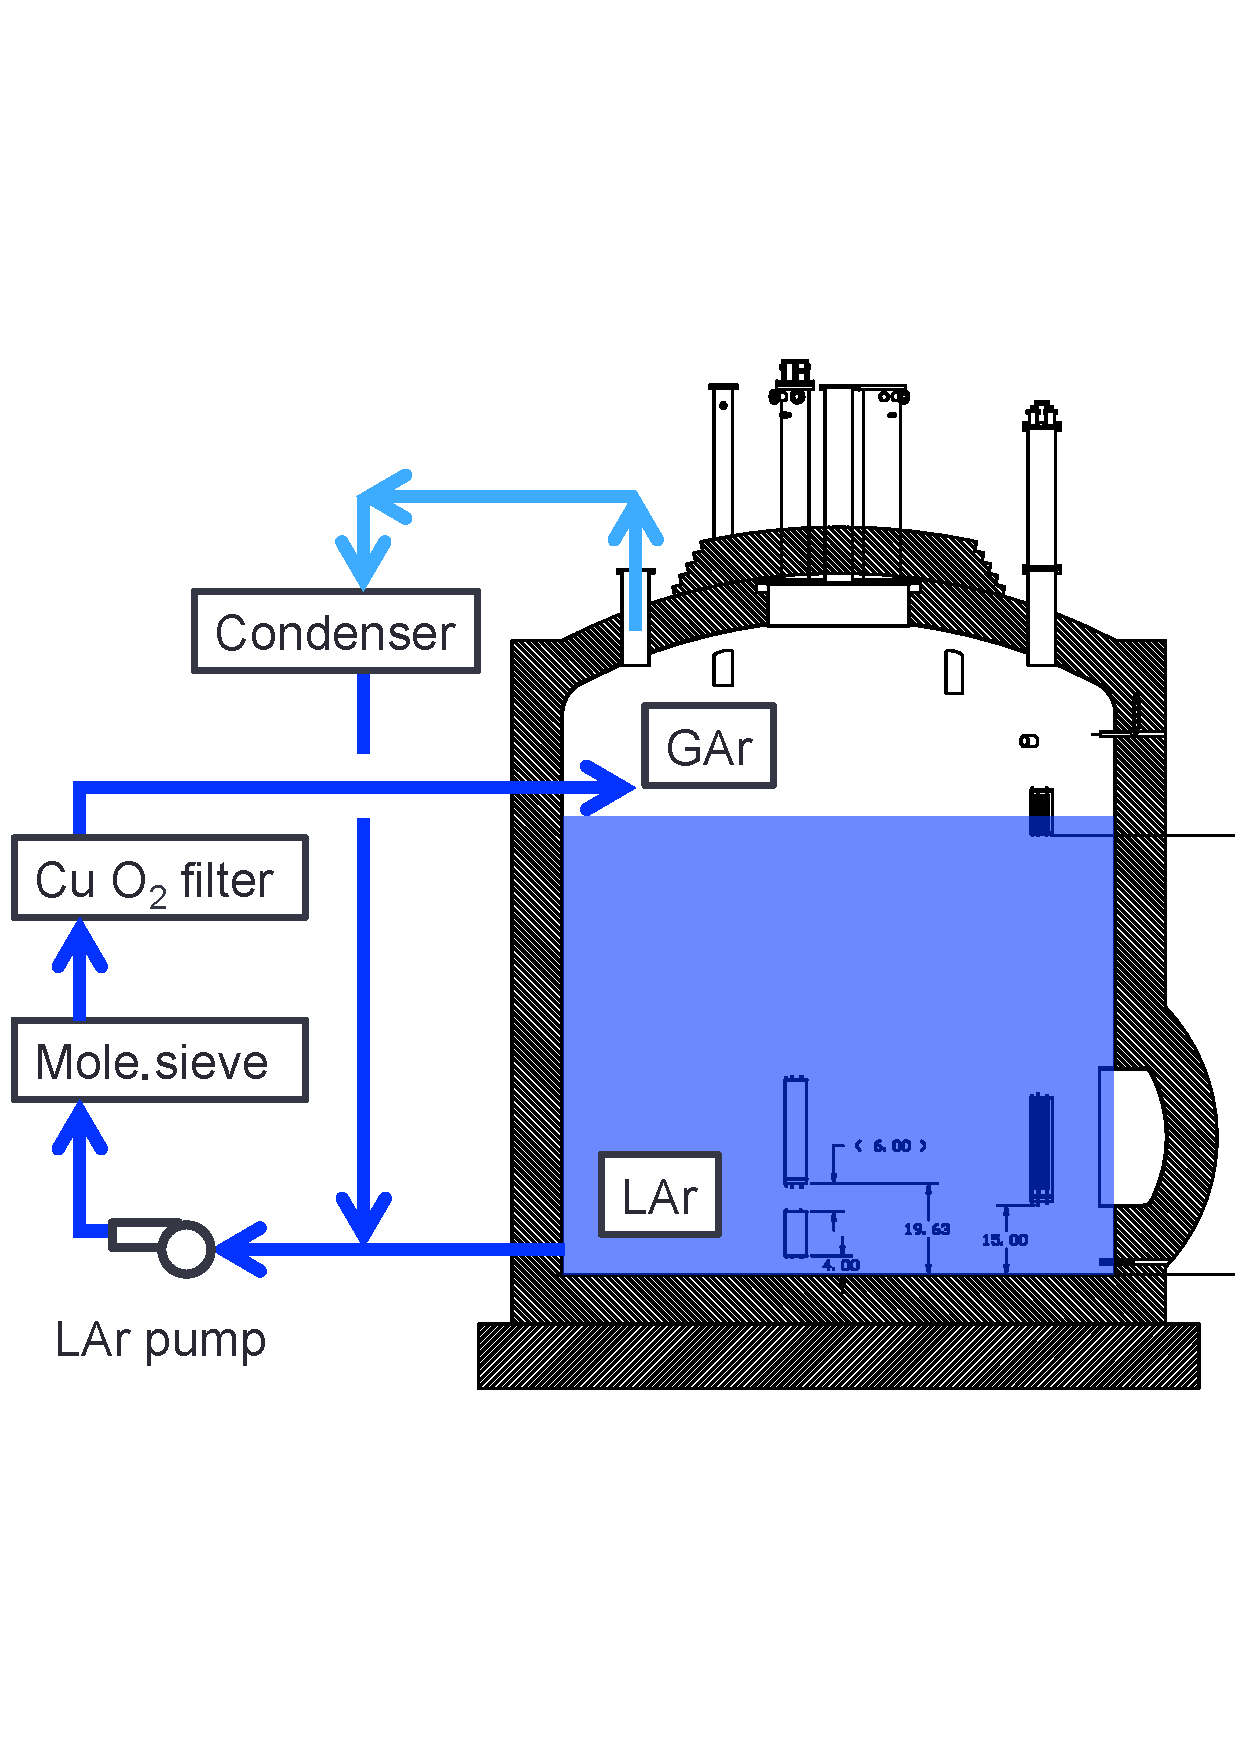
\includegraphics[width=10cm]{LAPDLiquidCirculation.pdf}
  \caption[Schematic showing the recirculation of the LAr during commissioning and operations of the Liquid Argon Purity Denomstrator.]{Schematic showing the recirculation of the LAr during commissioning and operations of the Liquid Argon Purity Denomstrator \cite{LAPD2014}.  Liquid is extracted from the bottom of the cryostat and pumped through the filters to remove any impurities which may have established in the medium.  Following the experience of previous R\&D with the MTS \cite{MTS2009a}, the recondensed liquid is passed through the purification system before being reintroduced to the main volume inside the cryostat.}
  \label{fig:LAPDLiquidCirculation}
\end{figure}

\subsubsection{LAPD Outcomes}\label{sec:LAPDOutcomes}

LAPD successfully demonstrated achieving and maintaining the required LAr purity for a large neutrino detector is possible without the costly and challenging use of evacuation techniques, reaching purities upwards of 60~ppt O$_2$ equivalent.  The measured electron lifetimes over the course of a six week run is shown in Figure~\ref{fig:LAPDElectronLifetime}.  Lifetimes of up to 4~ms were recorded, greater than the DUNE requirement of 3~ms although utlitising a much smaller-scale cryostat.  Nonetheless, the success of LAPD has great significance for future LArTPCs, including the 35~ton, and was an important stage in the FNAL LAr test program.

\begin{figure}[ht]
  \centering
  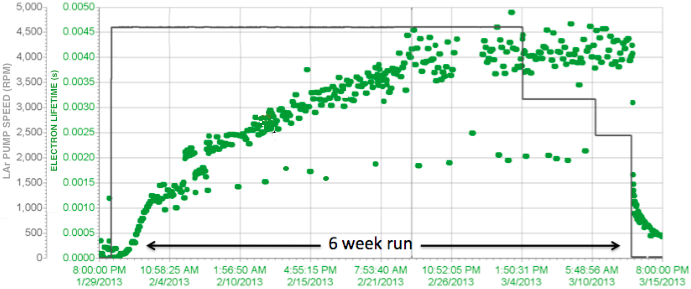
\includegraphics[width=12cm]{LAPDElectronLifetime.png}
  \caption[The electron lifetime achieved in the Liquid Argon Purity Demonstrator during a six week run.]{The electron lifetime achieved in the Liquid Argon Purity Demonstrator during a six week run.  Adapted from \cite{LAPD2014}.}
  \label{fig:LAPDElectronLifetime}
\end{figure}

\subsection{LongBo}\label{sec:LongBo}

Following the successful LAPD runs, a futher phase involved the introduction of a small-scale TPC detector into the liquid argon \cite{LongBo2015}.  The detector is named LongBo (an upgrade from the smaller Bo test detector) and is cylindrical with 25~cm diameter and 2~m length.  It was positioned vertically in the LAPD cryostat, demonstrated in Figure~\ref{fig:LongBo}, and was equipped with a high voltage on the cathode to produce the drift field and three wire planes at the top of the detector for readout.  External scintillator counters were placed around the outer wall of the cryostat to provide triggers on through-going cosmic muons which may deposit charge in the detector.

\begin{figure}
  \centering
  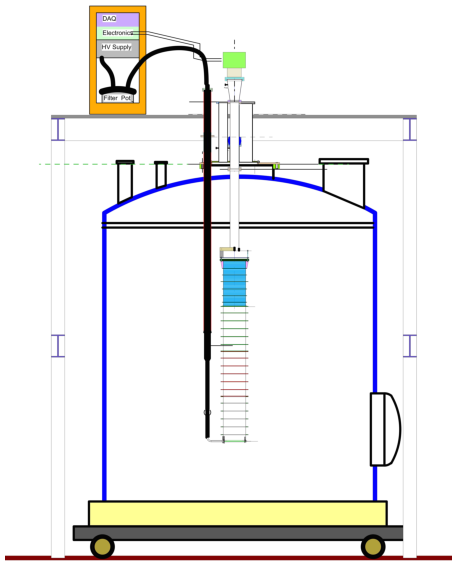
\includegraphics[width=8cm]{LongBo.pdf}
  \caption[The LongBo TPC detector shown within the Liquid Argon Purity Demonstrator Cryostat.]{The LongBo TPC detector shown within the Liquid Argon Purity Demonstrator Cryostat \cite{LongBo2015}.  The black tube represents the high voltage feedthrough to the cathode at the bottom of the TPC.}
  \label{fig:LongBo}
\end{figure}

LongBo was the first LArTPC experiment to utilise `cold readout' electronics to amplify and shape the signal at the front end.  An early version of the ASICs being developed for MicroBooNE were used to read out 16 of the 144 channels with the remaining using preamplifiers made with discrete circuitry.  At the drift field of 350~V/cm, the signal/noise ratio, a useful number in quantifying the electronics, was around 30, with the channels read out by the ASICs reporting values up to 1.4 times larger.

The LAPD/LongBo experiment successfully maintained similar LAr purities than without the presence of the detector, as predicted by the results of the MTS.  By using TPC data, it was also possible to make measurements of the electron lifetime from through-going muons (using Equation~\ref{eq:ElectronLifetime}).  A comparison between the measured values from the purity monitors and the TPC data may be found in Figure~\ref{fig:LongBoPurity}.  A reasonable agreement is observed between these complimentary measurements with values between 6~ms and 14~ms reported, with 95\% confidence.  These promising results confirmed designing and operating a LArTPC within a non-evacuable cryostat is viable and contributed to the development of the LAr program towards the DUNE far detector, with the 35~ton experiment the next stage.

\begin{figure}
  \centering
  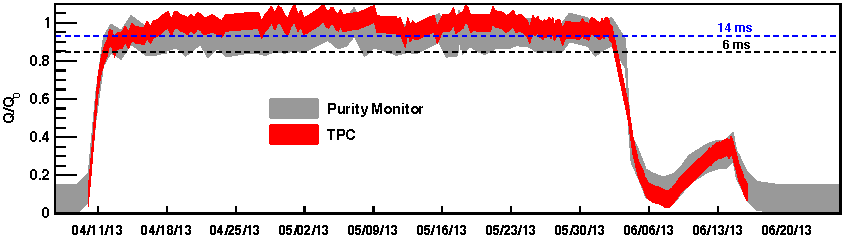
\includegraphics[width=14cm]{LongBoPurity.pdf}
  \caption[The LAr purity within the Liquid Argon Purity Demonstrator cryostat with the LongBo TPC present, measured using both data from the detector and information from the purity monitors.]{The LAr purity within the Liquid Argon Purity Demonstrator cryostat with the LongBo TPC present, measured using both data from the detector and information from the purity monitors \cite{LongBo2015}.}
  \label{fig:LongBoPurity}
\end{figure}

\section{35~ton Experiment: Phase I}\label{sec:35tonPhaseI}

The scale of the cryostats required for the DUNE experiment are such that constructing them as flat plane vessels 1.5~km underground would be unfeasibily expensive and pose huge engineering challenges.  Following the success of LAPD (discussed in Section~\ref{sec:LAPD}), which eliminates the requisite to evacuate the cryostat prior to filling, the LBNE collaboration decided to utilise membrane cryostat technology well established in the liquified natural gas (LNG) industry.  The 35~ton \cite{35tonPhaseI2014Cryostat,35tonPhaseI2014,35tonPhaseI2015} was therefore employed to demonstrate the application of a membrane cryostat to a LAr experiment and was the only planned prototype for LBNE.  The DUNE project has maintained this design choice and the 35~ton has since become a recognised and integral part of the collaboration, providing the first test of the technologies envisioned for the eventual far detector.

The 35~ton croystat was constructed in 2012 at PC4, a former proton facility in a decomissioned beamline, at Fermilab.  It has operated in two phases: Phase I (December 2013 -- February 2014) was proposed to demonstrate the membrane cryostat technology with just the cryostat and purification systems; Phase II (February 2016 -- April 2016) contained a small-scale DUNE-style detector to validate the integrated system and affirm the detector design elements.  The Phase I run is the subject of Section~\ref{sec:35tonPhaseI} whilst Phase II is considered in detail in Section~\ref{sec:35tonPhaseII}.

The 35~ton is the first membrane cryostat used for scientific purposes and the first overall constructed in the United States.  It is also the first designed to contain LAr, which is around three times denser than LNG.  The initial aims of the project (Phase I) include to demonstrate the feasibility of the cryostat technology for LAr, including thermal performance and leak tightness, and to show the required LAr purity may be acheived without evacuation and maintained through the use of the filtration system developed and validated by the MTS and LAPD.  This first phase will be discussed in this section; the 35~ton cryostat and filling procedures will be described in Sections~\ref{sec:35tonCryostat} and~\ref{sec:35tonFilling} respectively before outcomes of the experiment are presented in Section~\ref{sec:35tonPhaseIOutcomes}.

\subsection{The 35~ton Cryostat}\label{sec:35tonCryostat}

An overview of the 35~ton cryostat is shown in Figure~\ref{fig:35tonCryostat}.  It contains a concrete shell within which the membrane cryostat is constructed from 2~mm think stainless steel panels.  An insulated region between these two segments reduces heat leaking.  The roof consists of two plates; Plate A is flat with insulation and membrane beneath and Plate B contains all penetrations and services.  Relevant properties of the 35~ton cryostat are listed in Table~\ref{tab:35tonCryostat}.

\begin{figure}
  \centering
  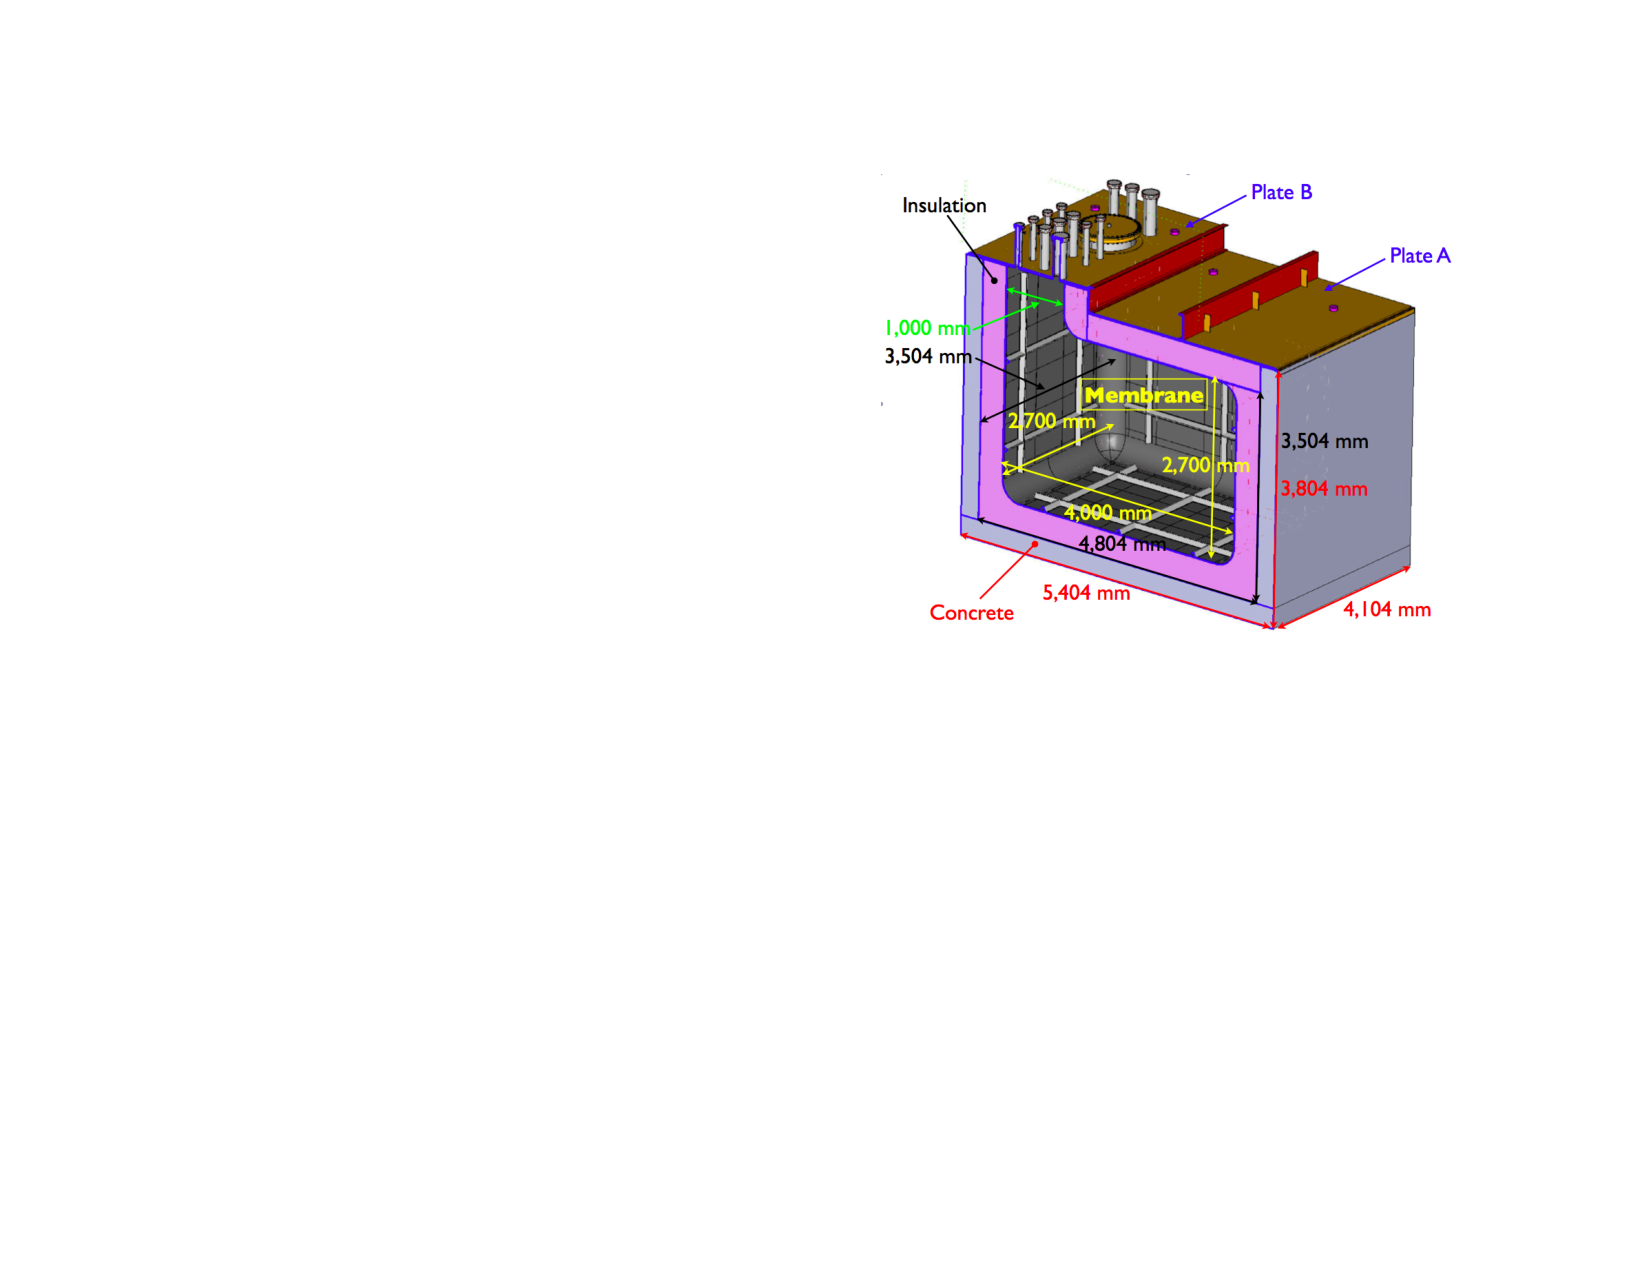
\includegraphics[width=10cm]{35tonCryostat.pdf}
  \caption[The 35~ton cryostat.]{The 35~ton cryostat \cite{35tonPhaseI2015}.}
  \label{fig:35tonCryostat}
\end{figure}

\begin{table}
  \caption[Details and dimensions of the 35~ton cryostat.]{Details and dimensions of the 35~ton cryostat \cite{35tonPhaseI2015}.}
  \label{tab:35tonCryostat}
  \centering
  \begin{tabular}{ l l }
    \toprule
    Parameter & Value \\
    \midrule
    Cryostat volume           & 29.16~m$^3$ \\
    LAr total mass            & 38.6~metric tons \\
    Depth of LAr              & 2.565~m (11\% total ullage) \\
    Inner dimensions          & 4.0~m (length) $\times$ 2.7~m (width) $\times$ 2.7~m (height) \\
    Insulation                & 0.4~m polyurethane foam \\
    Primary membrane          & 2.0~mm thick corrugated stainless steel \\
    Secondary barrier system  & 0.1~mm thick fiberglass \\
    Vapor barrier             & 1.2~mm thick carbon steel \\
    Steel reinforced concrete & 0.3~m thick layer \\
    LAr temperature           & $89\pm1$~K \\
    Operating gas pressure    & 70~mBar \\
    Design pressure           & 207~mBar \\
    Heat leak                 & $<13$~W/m$^2$ \\
    Leak tightness            & $1\times10^{-6}$~mBar$\cdot$litre/s \\
    \bottomrule
  \end{tabular}
\end{table}

The 35~ton was constructed physically nearby the Liquid Argon Purity Demonstrator in order to utilise existing infrastructure.  It is connected to the LAPD tank, which may be used to store LAr before transferring to the 35~ton, and uses the filtration setup designed and validated by the MTS and LAPD.  This network is shown schematically in Figure~\ref{fig:35tonLAPD}.  Unlike in LAPD, the pumps used in the 35~ton to circulate the LAr through the purification system are within the liquid but the framework operates in a similar way.  An identical condenser is also employed above the cryostat to cool boiled off gaseous argon which is returned to the bottom of the cryostat, nearby the pumps which subsequently extract the liquid for purification.

\begin{figure}
  \centering
  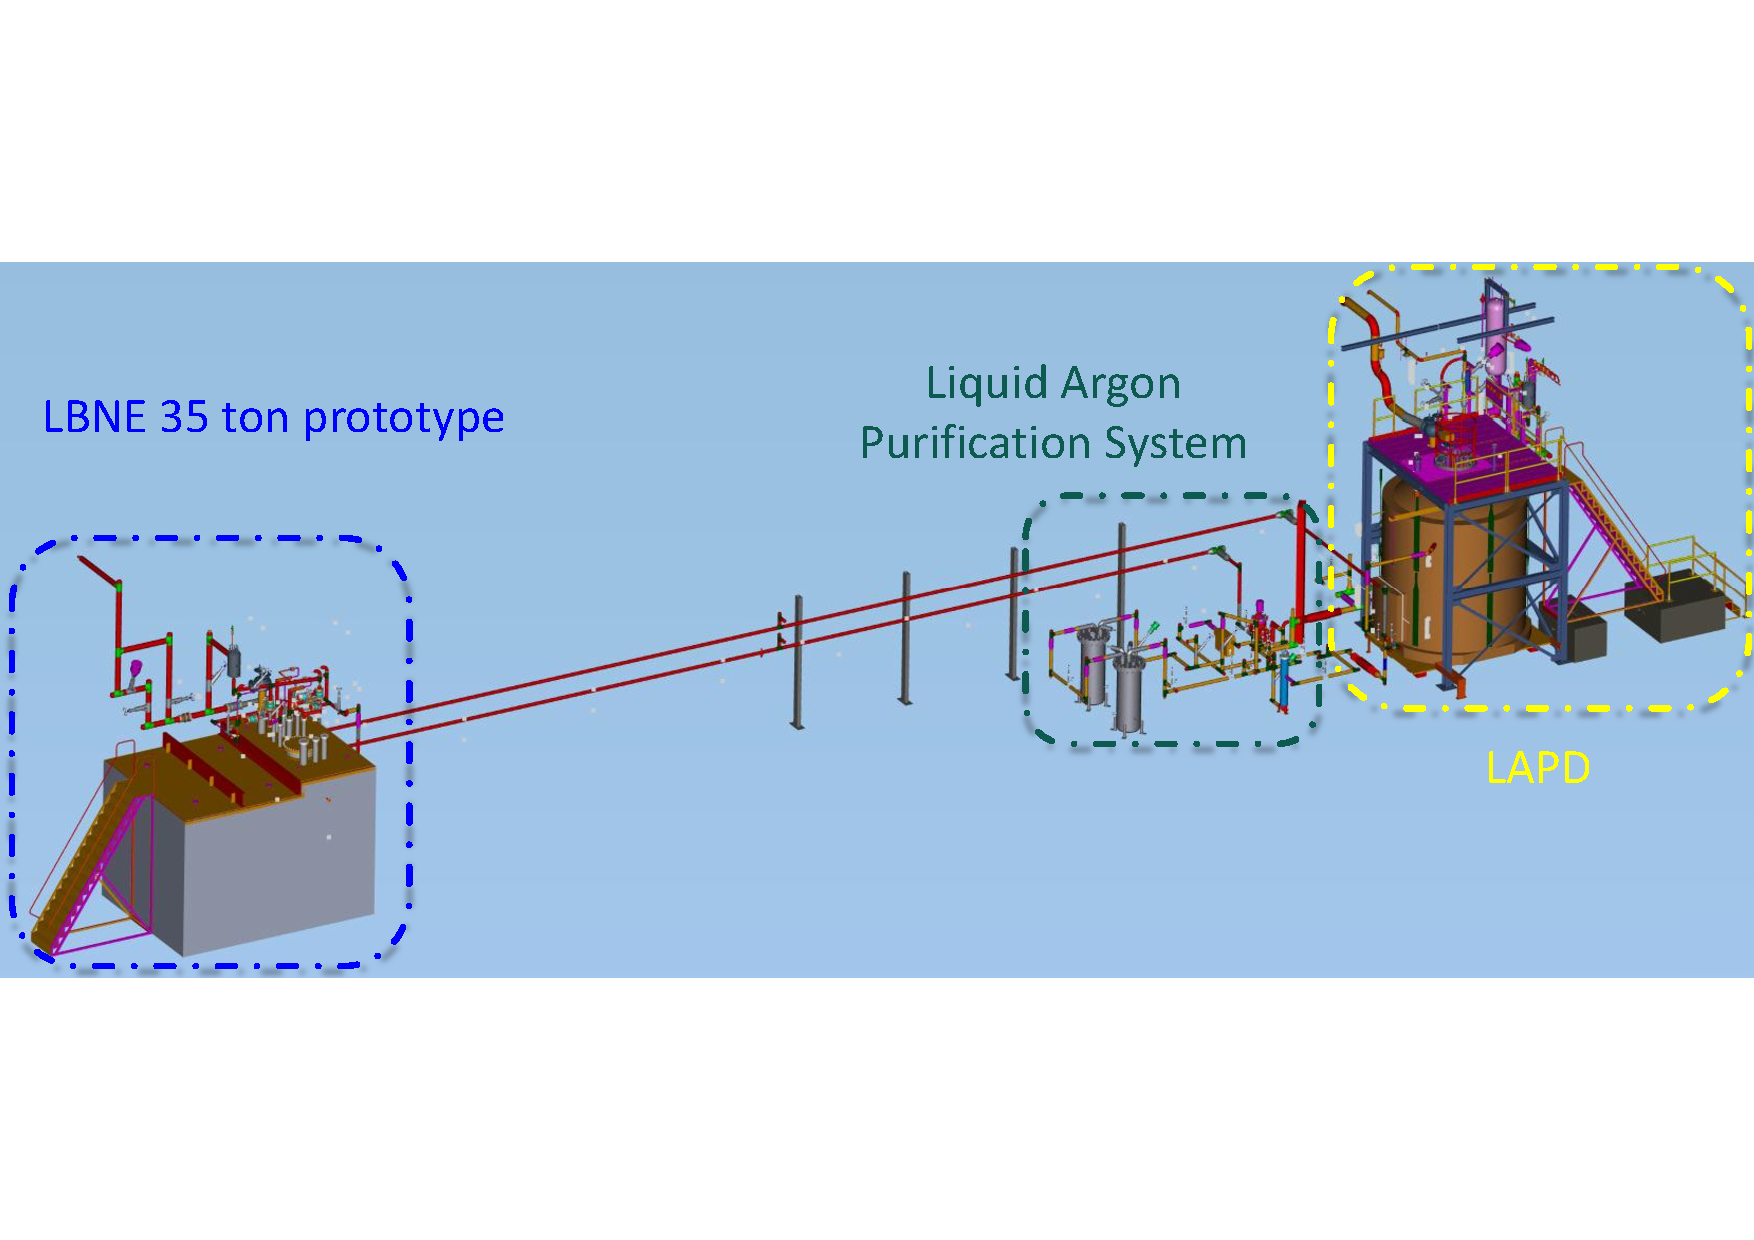
\includegraphics[width=14cm]{35tonLAPD.pdf}
  \caption[The network linking the 35~ton cryostat, the Liquid Argon Purity Demonstrator and the purification system at PC4, Fermilab.]{The network linking the 35~ton cryostat, the Liquid Argon Purity Demonstrator and the purification system at PC4, Fermilab \cite{35tonPhaseI2014}.}
  \label{fig:35tonLAPD}
\end{figure}

The cryogenic environment is monitored and controlled using standard detectors including temperature sensors, pressure transducers, flow meters and level sensors along with a suite of commercial gas analysers.  The height of the volume is instrumented with four purity monitors, two large and two small, with an additional long monitor positioned after the filters, as with LAPD.  Also as previously, the vertical temperature profile in the cryostat is monitored at 23~cm intervals with temperature detectors suspended on a chain.

\subsection{Filling the 35~ton}\label{sec:35tonFilling}

The 35~ton cryostat is filled in a similar way to the Liquid Argon Purity Demonstrator, described in Section~\ref{sec:FillingLAPD}.  Initially, a piston purge with warm gaseous argon is performed to remove atmospheric impurities before closing off the vents and redirecting argon at the top of the cryostat through the filters for purification.  The impurity concentrations for this stage of filling are shown in Figure~\ref{fig:35tonGasFilling}.  Before filling with liquid, the cryostat is cooled in an attempt to reduce outgassing and to create an appropriate environment in which to introduce LAr.  This is achieved by injecting LAr through a spray at the top of the cryostat which generates a turbulent mixing of cold gas within the cryostat and gradually cools the walls of the vessel.  Following this, LAr is transferred from LAPD into the 35~ton; this is conducted in two stages since the 35~ton is slightly larger than LAPD.  The cooldown and LAr filling stages are shown in Figure~\ref{fig:35tonLiquidFilling}.

\begin{figure}
  \centering
  \begin{subfigure}[t]{0.48\linewidth}
    \centering
    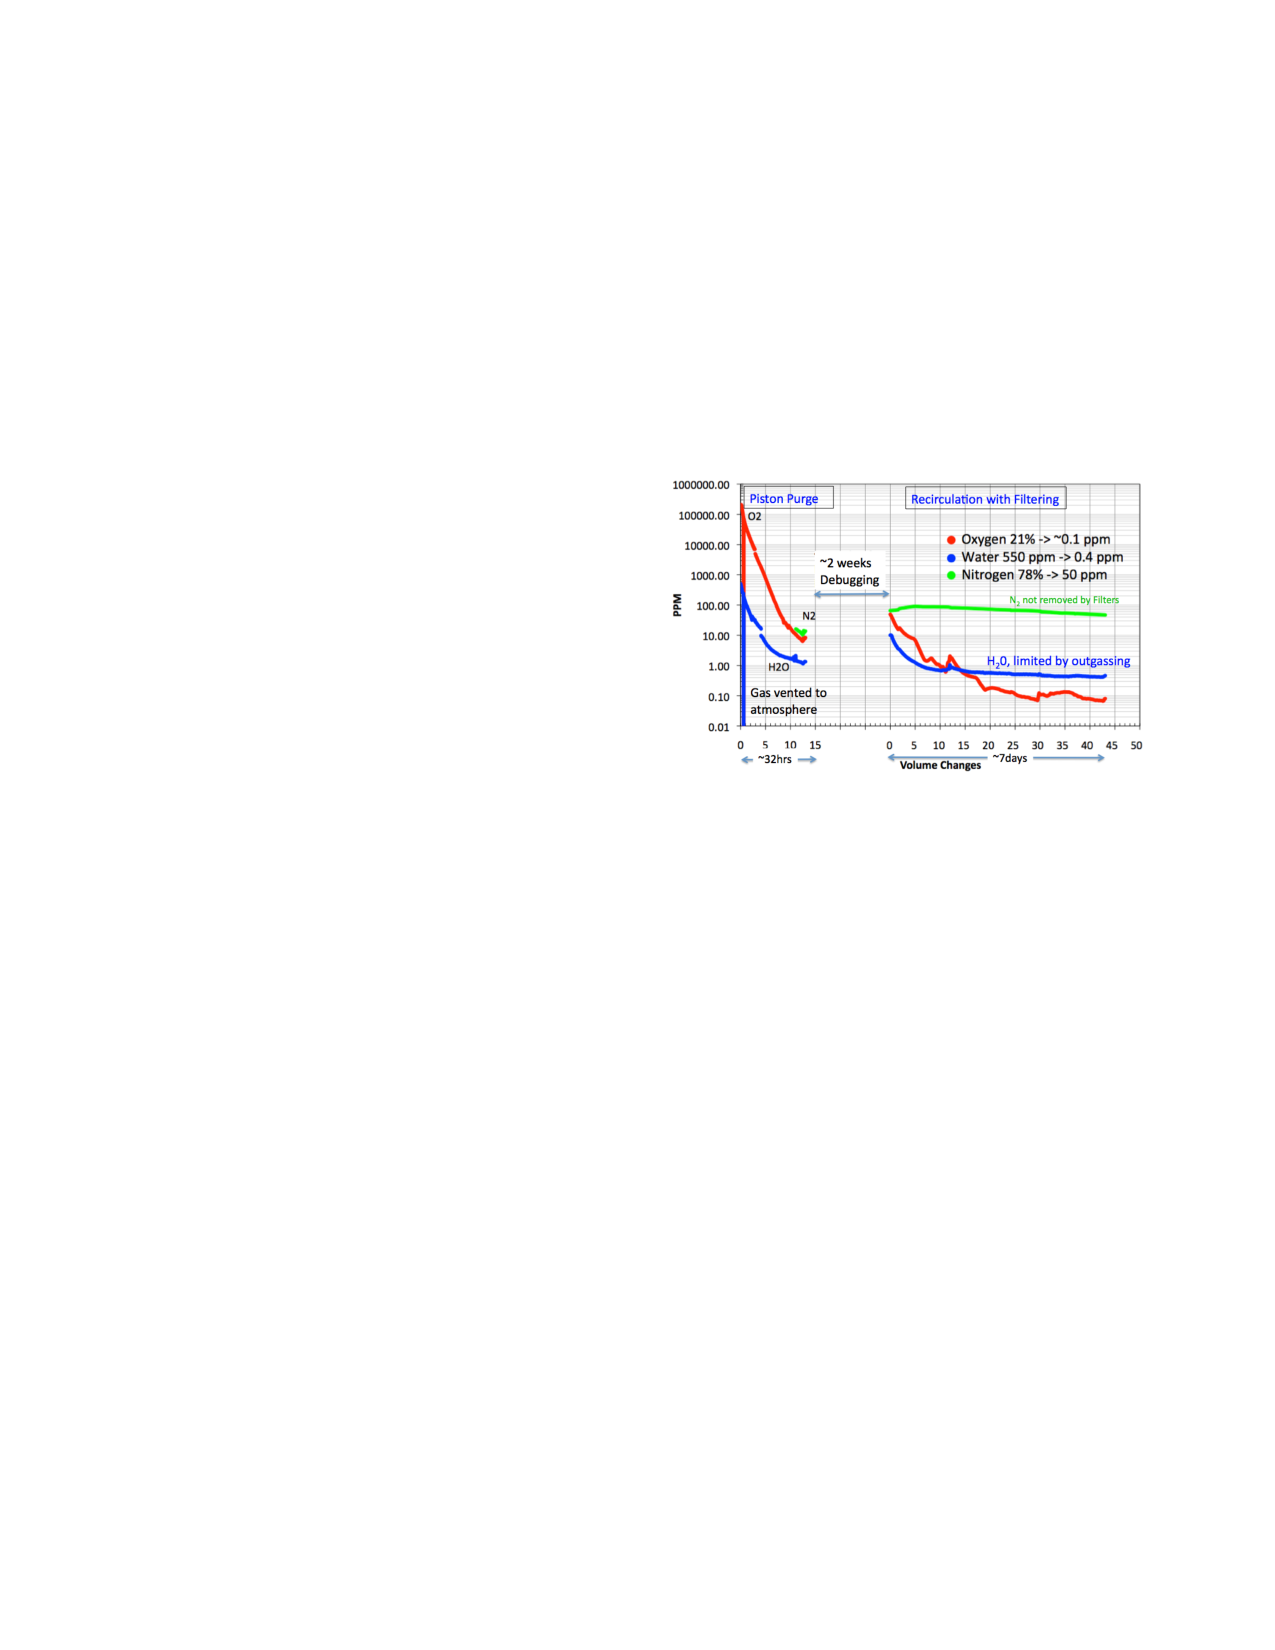
\includegraphics[width=0.98\textwidth]{35tonGasFilling.pdf}
    \caption{Gas filling.}
    \label{fig:35tonGasFilling}
  \end{subfigure}
  \hfill
  \begin{subfigure}[t]{0.48\linewidth}
    \centering
    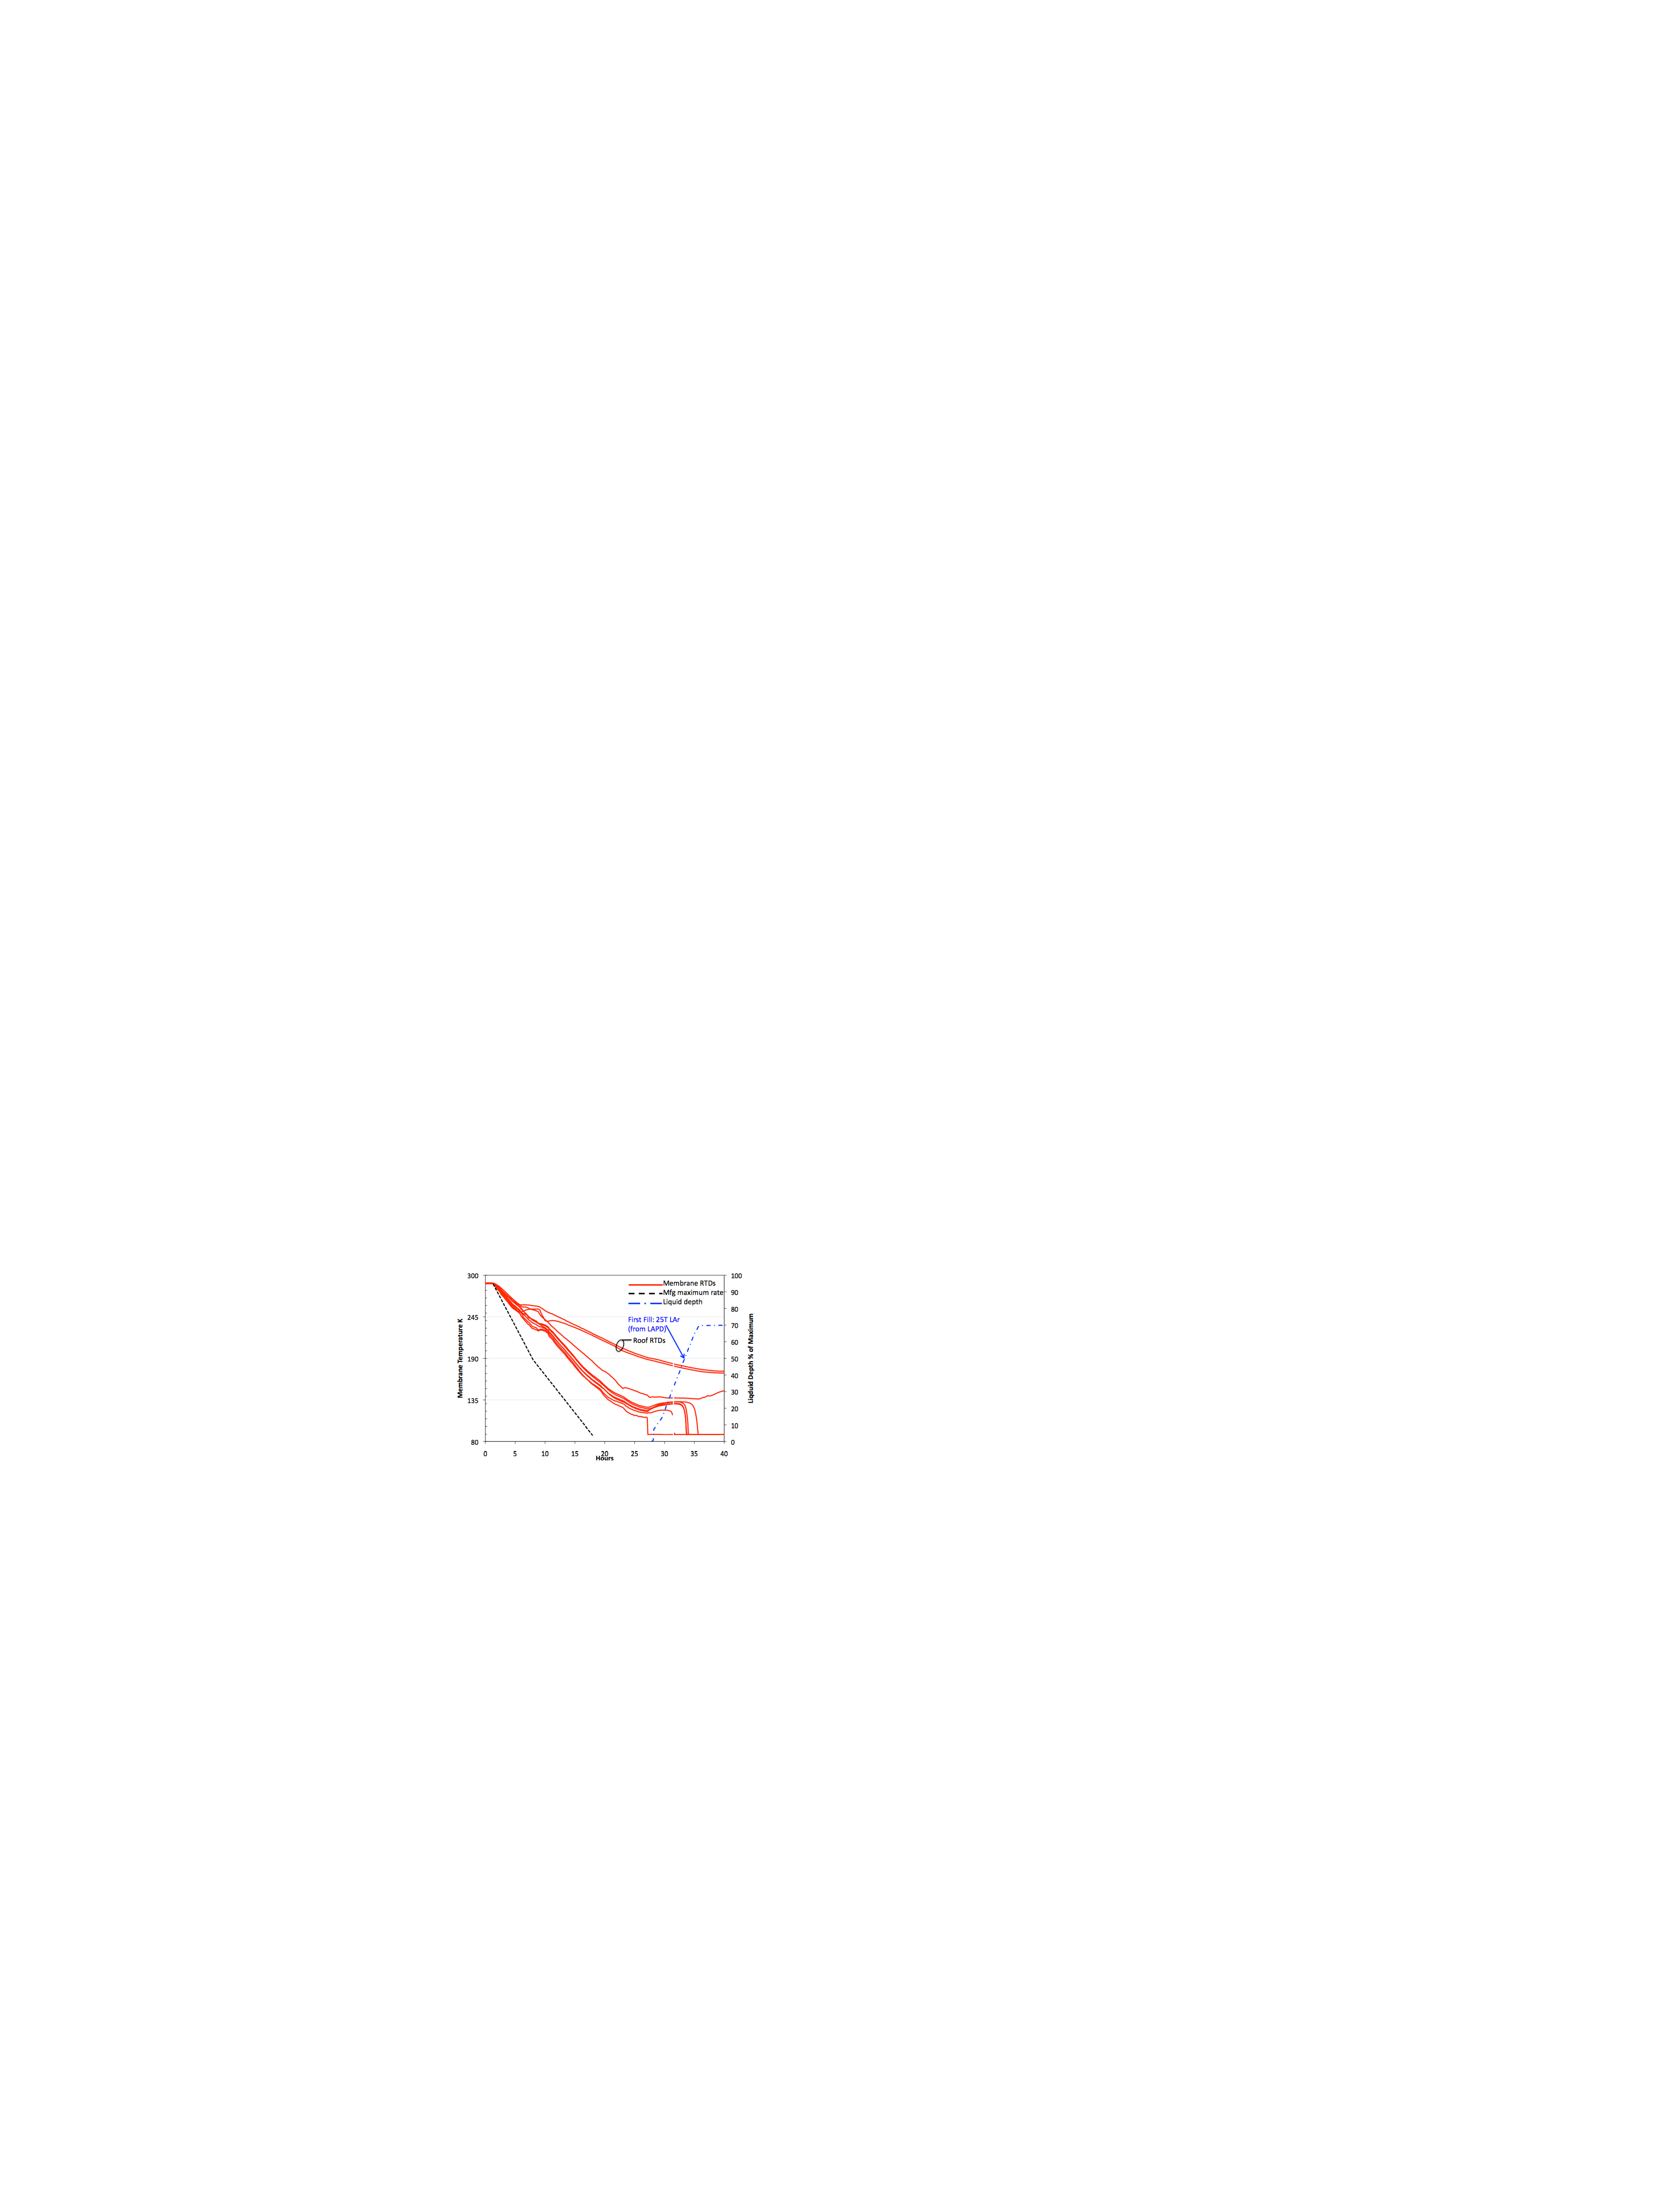
\includegraphics[width=0.98\textwidth]{35tonLiquidFilling.pdf}
    \caption{Liquid filling.}
    \label{fig:35tonLiquidFilling}
  \end{subfigure}
  \caption[Filling the 35~ton cryostat in four stages: piston purge, gas recirculation, cooldown and liquid filling.]{Filling the 35~ton cryostat in four stages: piston purge, gas recirculation, cooldown, liquid filling \cite{35tonPhaseI2015}.  The gas filling is shown in Figure~\ref{fig:35tonGasFilling} and involves using a piston purge to fill the tank with warm gaseous argon before circulating this gas through the filtration system.  Cooldown and liquid filling is demonstrated in Figure~\ref{fig:35tonLiquidFilling}, which shows the falling temperature of the crysotat as a result of the injection of liquid argon through the cooldown sprayers and the rising LAr level as the cryostat is filled from LAPD.}
  \label{fig:35tonFilling}
\end{figure}

\subsection{Outcomes of Phase I}\label{sec:35tonPhaseIOutcomes}

The 35~ton successfully demonstrated the feasibility of membrane cryostats for use with LAr and additionally showed the required LAr purity for future multi-kton LArTPC experiments may be achieved and held in such a vessel.  The lifetime over the course of the $\sim2$~month run, along with external changes to the system, is comprehensively summarised in Figure~\ref{fig:35tonPhaseIElectronLifetime}.

\begin{figure}
  \centering
  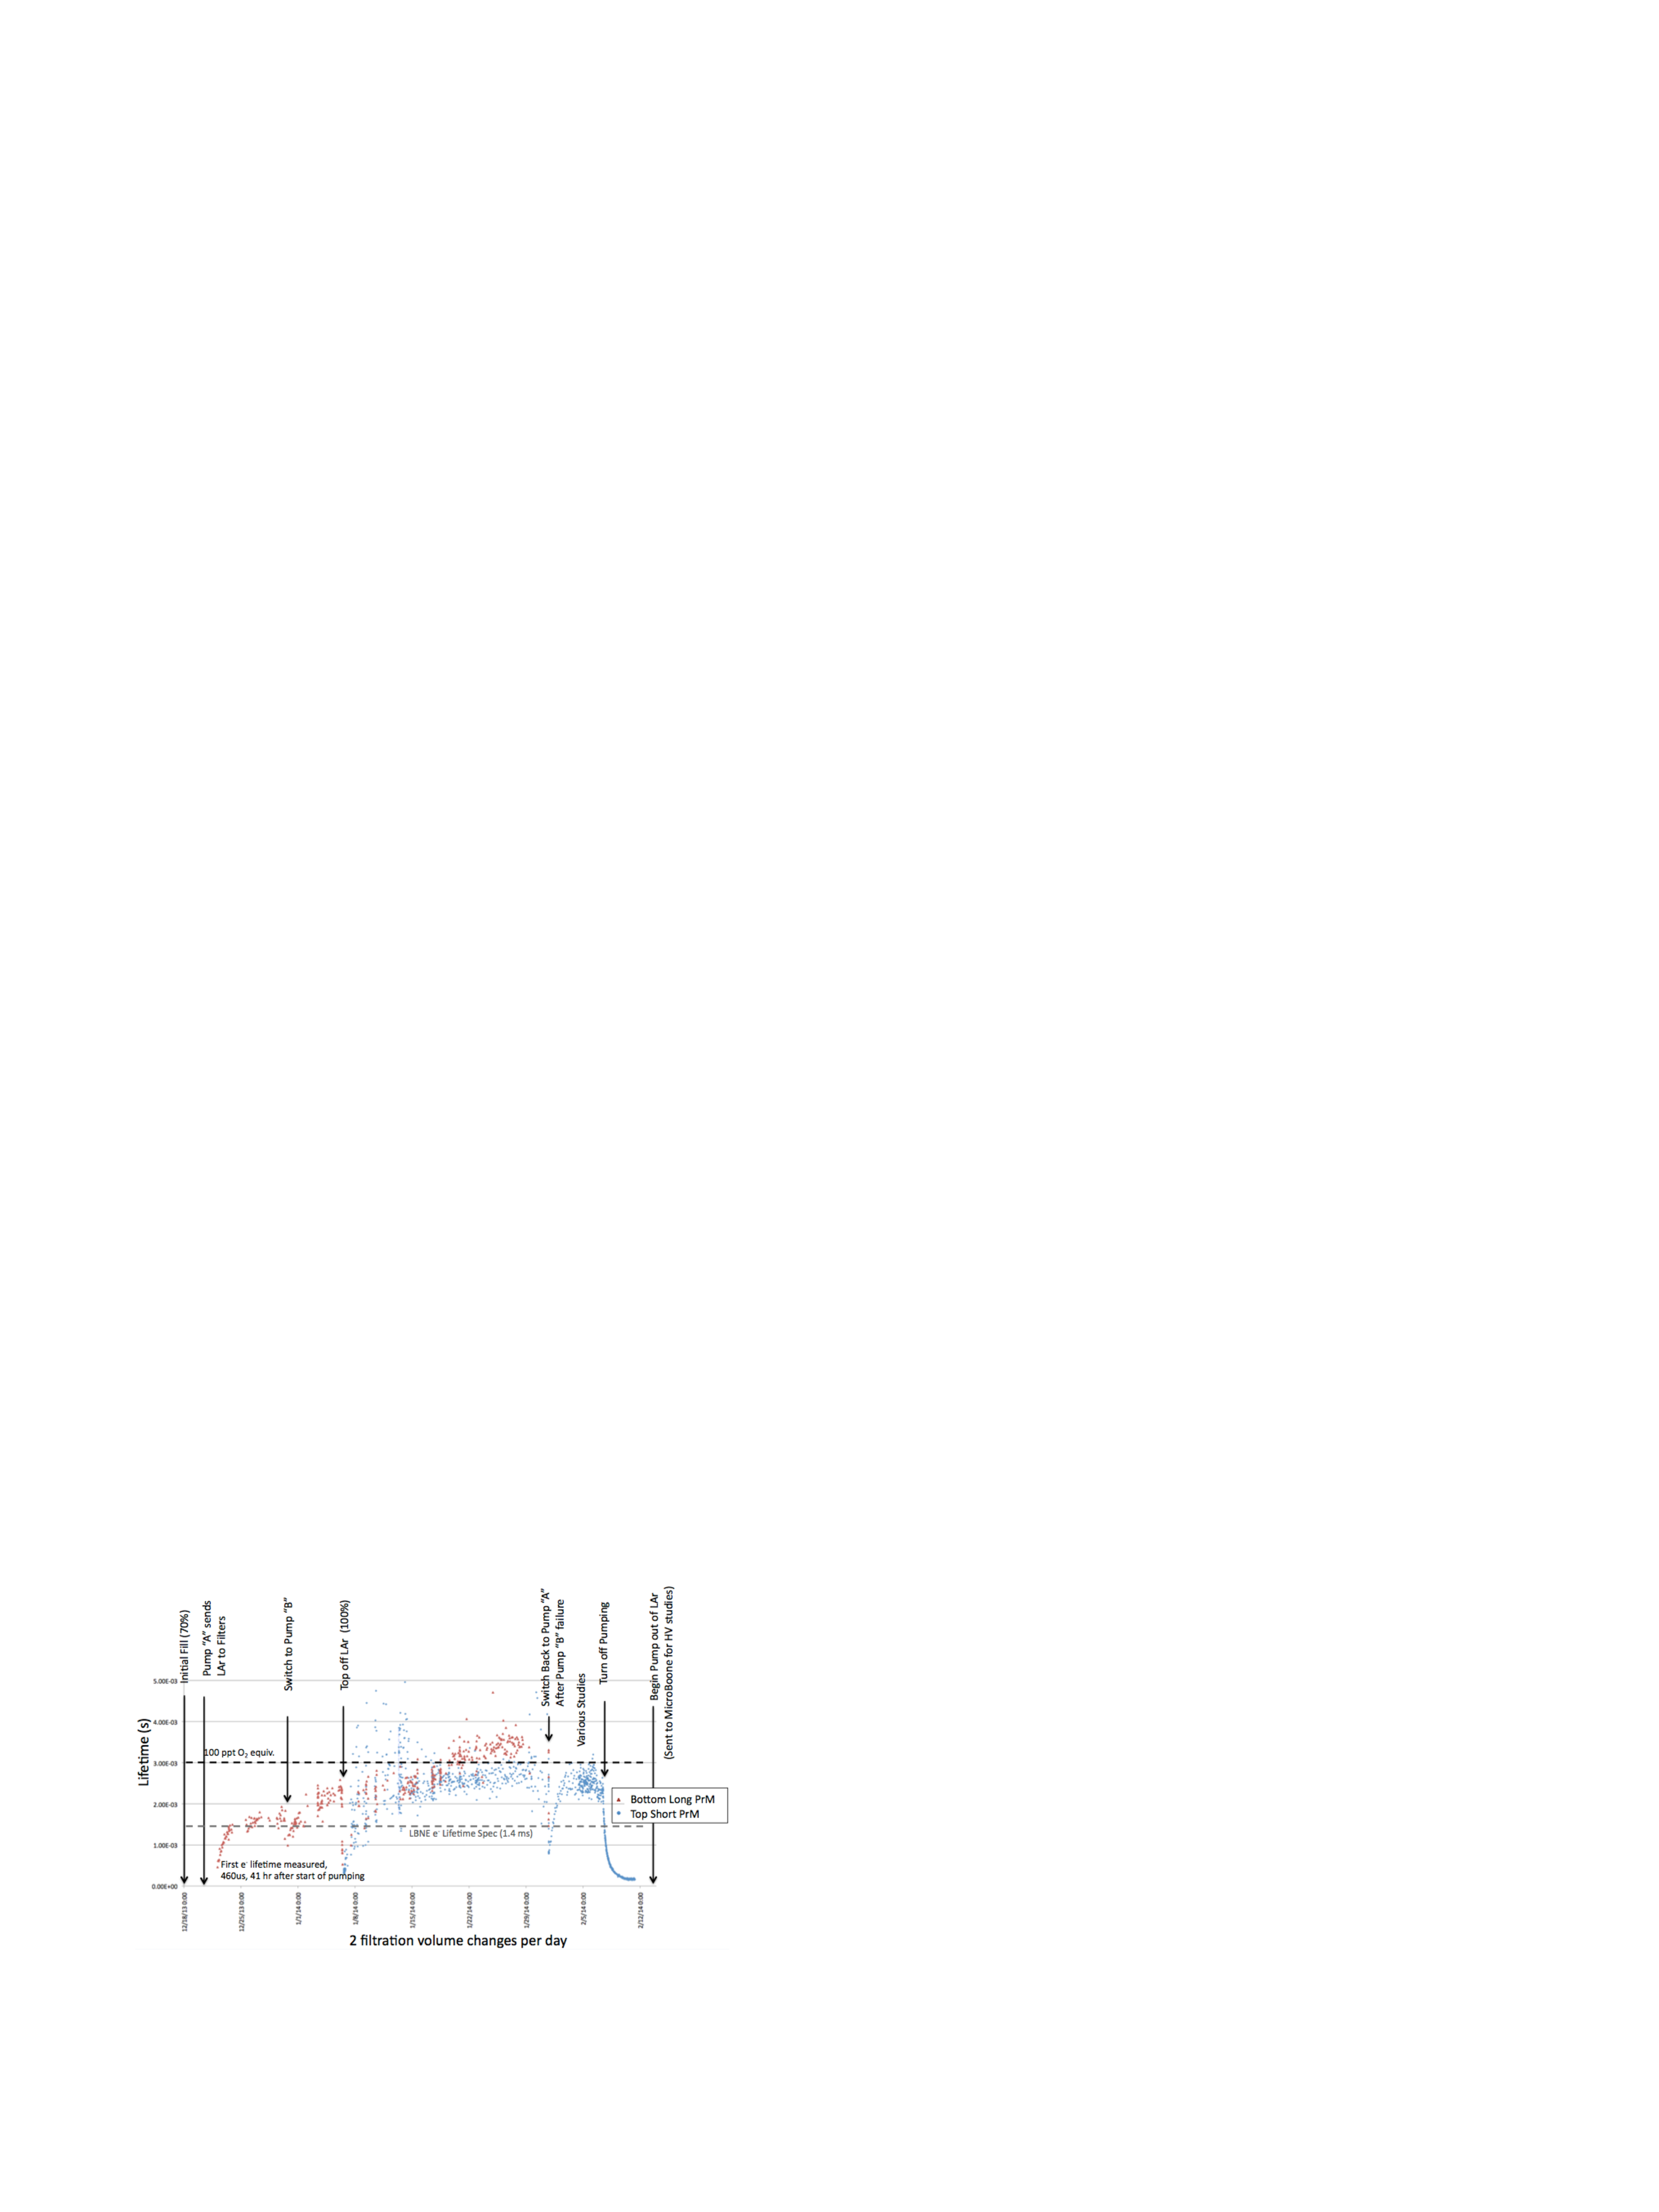
\includegraphics[width=14cm]{35tonPhaseIElectronLifetime.pdf}
  \caption[The electron lifetime in the 35~ton cryostat measured by two purity monitors over the course of the two month Phase I run.]{The electron lifetime in the 35~ton cryostat measured by two purity monitors over the course of the two month Phase I run \cite{35tonPhaseI2014}.  The measurements correspond to different positions in the cryostat, with the red points showing purity measurements at the bottom and blue points near the top.  Major external factors affecting the observed LAr purity are shown at the top of the figure.  The old LBNE requirement of 1.4~ms is noted as a dashed grey line; DUNE now requires 3~ms lifetime, equivalent to 100~ppt O$_2$ equivalent and illustrated by the black dashed line.}
  \label{fig:35tonPhaseIElectronLifetime}
\end{figure}

The lifetime is observed to reach and remain at the DUNE requirement for a good period of time; this is a major achievement in the context of the future of LArTPC experiments.  Dips in the purity were observed when topping up the croystat after initially filling one LAPD volume and when switching between the two pumps installed to extract the liquid for purification.  In both cases, good purity is recovered after a few volume exchanges.

The same variations of lifetime on temperature were observed as previously noted in the MTS and LAPD, suggesting a genuine effect dependent on the ambient conditions.  Addtionally, during gas circulation a leak was found and fixed in a seal and, during cold operations, a leak developed in the argon cryo-piping as the dielectric breaks necessary to electrically isolate the cryostat from the building were not leak tight at cryogenic temperatures.  All associated 35~ton experience is useful as progress continues to larger and more complicated LAr cryostats.

The success of the 35~ton was exploited by utilising the existing setup for a second run, involving a small-scale DUNE-style detector.  This would be the first time a membrane cryostat would facilitate a detector and is the next stage along in prototyping the DUNE far detector.

\section{35~ton Experiment: Phase II}\label{sec:35tonPhaseII}

Time for phase II!

\subsection{The 35~ton Detector}

\subsubsection{TPC}

\subsubsection{Photon Detectors}

\subsubsection{External Counters}

\subsection{Data Acquisition}

\subsubsection{RCEs, SSPs, PTB}

\subsubsection{35~ton DAQ}

\subsection{The Sheffield Camera System}

\subsection{Data Taking}

\subsection{Outcomes of Phase II}

\section{Summary}\label{sec:35tonSummary}

%% %------------------------------------------------------------------------------------------------------------------------------------------------------------
%% \section{The 35~ton Detector}\label{sec:35tonDetector}

%% In 35t, we have FE ASICs which are the very front end and apply the signal shaping and gain.  Have regulators to control the power these receive (these are noisy...).  Also ADC ASICs to do digitisation in the cold.  MicroBooNE don't do this, this just have the front end and do everything else in the warm.  FE ASICs are the problem, same for uBooNE and 35t.  ADC ASIC has stuck code problem.

%% \subsection{Detector Components}\label{sec:35tonDetectorComponents}

%% \subsubsection{TPC}\label{35tonTPC}

%% \subsubsection{Photon Detectors}\label{sec:35tonPhoton}

%% \subsubsection{External Counters}\label{sec:35tonCounters}

%% \subsection{Readout Electronics}\label{sec:35tonReadoutElectronics}

%% \subsubsection{FEMBs}\label{sec:35tonFEMB}

%% \subsubsection{RCEs}\label{sec:35tonRCE}

%% \subsubsection{SSPs}\label{sec:35tonSSP}

%% \subsubsection{PTB}\label{sec:35tonPTB}

%% \subsection{DAQ}\label{sec:35tonDAQ}

%% %------------------------------------------------------------------------------------------------------------------------------------------------------------
%% \section{Filling the 35~ton}\label{sec:35tonFilling}

%% %------------------------------------------------------------------------------------------------------------------------------------------------------------
%% \section{The 35~ton Experimental Setup}\label{sec:35tonExperiment}

%% \subsection{Filtration System}\label{sec:35tonFiltration}

%% Same as LAPD.

%% \subsection{Purity Monitoring}\label{sec:35tonPurity}

%% Same as LAPD.

%% %------------------------------------------------------------------------------------------------------------------------------------------------------------
%% \section{35~ton Phase I}\label{sec:35tonPhaseI}

%% \subsection{Outcomes}\label{sec:35tonPhaseIOutcomes}

%% %------------------------------------------------------------------------------------------------------------------------------------------------------------
%% \section{35~ton Phase II}\label{sec:35tonPhaseII}

%% \subsection{Commissioning}\label{sec:35tonCommissioning}

%% \subsection{The Sheffield Camera System}\label{sec:35tonCameraSystem}

%% Wait for Nicola to finish the paper and plagerise!

%% \subsection{Online Monitoring for Data Quality Monitoring}\label{sec:35tonOnlineMonitoring}

%% \subsection{Outcomes}\label{sec:35tonPhaseIIOutcomes}
































%% % The very first part of my thesis, written June 2015.  I'll leave it here to remember it!

%% %% \section{The DUNE 35ton LAr Prototype}

%% %% The DUNE far detector (see section
%% %% %\ref{sec:DUNEFD})
%% %% has a very large, complicated design including many features which are novel to this experiment. In order to optimise and minimise potential complications during construction an\
%% %% d commissioning, several levels of prototyping are necessary during the design. These include the membrane cryostat, a TPC within such a cryostat, full scale detector elements, \
%% %% installation test and complete vertical slice tests of all electronics. Many of these have been tested with the first of two DUNE prototypes, the 35-ton (ref Far Detector Extern\
%% %% al Review, May 19-20 2015).

%% %% There was a phase 1 run! \cite{LBNE35tonPhase1}

%% %% \subsection{Overview of the 35-ton}

%% %% The 35-ton is a

%% %% The 35~ton consists of a membrane cryostat (Section \ref{sec:35tonCryostat}), designed to be filled with 35 metric tons of liquid argon, and a small-scale DUNE-style detector (Section \ref{sec:35tonDetector}) including a TPC and photon detectors.  It was constructed in 2012 at PC4, a former proton facility in a decomissioned beamline, at Fermilab.  The Phase I run, without a detector, took place between December 2013 and February 2014.  Between February 2014 and September 2015 the detector was constructed and heavily tested at FNAL before being installed inside the cryostat ready for the Phase II run.  This took place between February 2016 and April 2016 (offically starting on 11th February, as I type!).

